% Created by tikzDevice version 0.12 on 2019-10-03 14:50:42
% !TEX encoding = UTF-8 Unicode
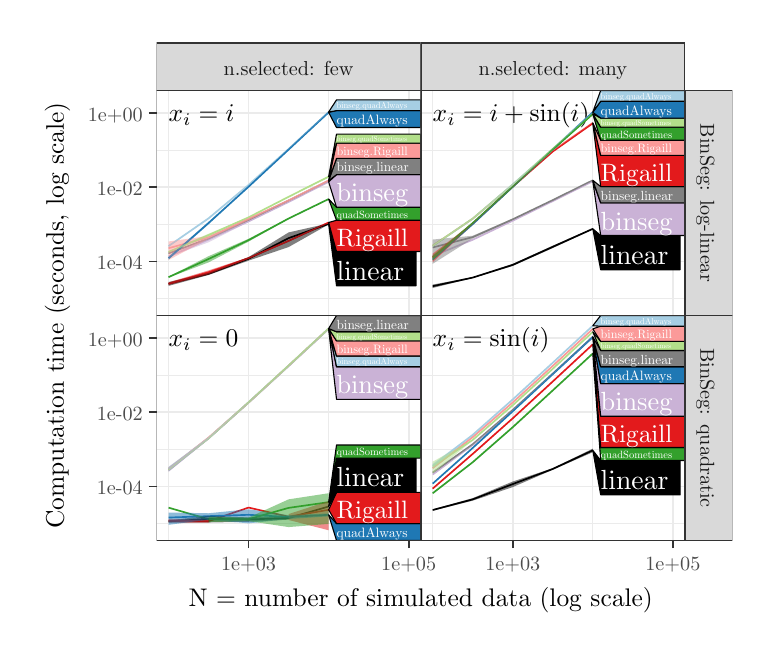
\begin{tikzpicture}[x=1pt,y=1pt]
\definecolor{fillColor}{RGB}{255,255,255}
\path[use as bounding box,fill=fillColor,fill opacity=0.00] (0,0) rectangle (260.17,216.81);
\begin{scope}
\path[clip] (  0.00,  0.00) rectangle (260.17,216.81);
\definecolor{drawColor}{RGB}{255,255,255}
\definecolor{fillColor}{RGB}{255,255,255}

\path[draw=drawColor,line width= 0.6pt,line join=round,line cap=round,fill=fillColor] (  0.00,  0.00) rectangle (260.17,216.81);
\end{scope}
\begin{scope}
\path[clip] ( 46.56,112.81) rectangle (142.02,194.12);
\definecolor{fillColor}{RGB}{255,255,255}

\path[fill=fillColor] ( 46.56,112.81) rectangle (142.02,194.12);
\definecolor{drawColor}{gray}{0.92}

\path[draw=drawColor,line width= 0.3pt,line join=round] ( 46.56,118.89) --
	(142.02,118.89);

\path[draw=drawColor,line width= 0.3pt,line join=round] ( 46.56,145.76) --
	(142.02,145.76);

\path[draw=drawColor,line width= 0.3pt,line join=round] ( 46.56,172.63) --
	(142.02,172.63);

\path[draw=drawColor,line width= 0.3pt,line join=round] ( 50.90,112.81) --
	( 50.90,194.12);

\path[draw=drawColor,line width= 0.3pt,line join=round] (108.75,112.81) --
	(108.75,194.12);

\path[draw=drawColor,line width= 0.6pt,line join=round] ( 46.56,132.33) --
	(142.02,132.33);

\path[draw=drawColor,line width= 0.6pt,line join=round] ( 46.56,159.20) --
	(142.02,159.20);

\path[draw=drawColor,line width= 0.6pt,line join=round] ( 46.56,186.07) --
	(142.02,186.07);

\path[draw=drawColor,line width= 0.6pt,line join=round] ( 79.83,112.81) --
	( 79.83,194.12);

\path[draw=drawColor,line width= 0.6pt,line join=round] (137.68,112.81) --
	(137.68,194.12);
\definecolor{drawColor}{RGB}{0,0,0}

\node[text=drawColor,anchor=base west,inner sep=0pt, outer sep=0pt, scale=  0.92] at ( 50.90,182.82) {$x_i = i$};
\definecolor{drawColor}{RGB}{202,178,214}

\path[draw=drawColor,line width= 0.6pt,line join=round] ( 50.90,134.11) --
	( 65.36,140.25) --
	( 79.83,146.80) --
	( 94.29,153.84) --
	(108.75,161.11);
\definecolor{drawColor}{gray}{0.50}

\path[draw=drawColor,line width= 0.6pt,line join=round] ( 50.90,135.25) --
	( 65.36,140.60) --
	( 79.83,147.38) --
	( 94.29,154.36) --
	(108.75,161.51);
\definecolor{drawColor}{RGB}{0,0,0}

\path[draw=drawColor,line width= 0.6pt,line join=round] ( 50.90,124.23) --
	( 65.36,127.87) --
	( 79.83,133.31) --
	( 94.29,140.76) --
	(108.75,145.90);
\definecolor{drawColor}{RGB}{251,154,153}

\path[draw=drawColor,line width= 0.6pt,line join=round] ( 50.90,137.12) --
	( 65.36,141.04) --
	( 79.83,147.66) --
	( 94.29,154.39) --
	(108.75,161.56);
\definecolor{drawColor}{RGB}{227,26,28}

\path[draw=drawColor,line width= 0.6pt,line join=round] ( 50.90,124.30) --
	( 65.36,128.42) --
	( 79.83,133.55) --
	( 94.29,139.77) --
	(108.75,146.41);
\definecolor{drawColor}{RGB}{166,206,227}

\path[draw=drawColor,line width= 0.6pt,line join=round] ( 50.90,137.88) --
	( 65.36,147.91) --
	( 79.83,160.00) --
	( 94.29,172.99) --
	(108.75,186.33);
\definecolor{drawColor}{RGB}{31,120,180}

\path[draw=drawColor,line width= 0.6pt,line join=round] ( 50.90,133.49) --
	( 65.36,146.22) --
	( 79.83,159.34) --
	( 94.29,172.76) --
	(108.75,186.21);
\definecolor{drawColor}{RGB}{178,223,138}

\path[draw=drawColor,line width= 0.6pt,line join=round] ( 50.90,135.79) --
	( 65.36,141.86) --
	( 79.83,148.27) --
	( 94.29,155.70) --
	(108.75,162.98);
\definecolor{drawColor}{RGB}{51,160,44}

\path[draw=drawColor,line width= 0.6pt,line join=round] ( 50.90,126.66) --
	( 65.36,133.21) --
	( 79.83,140.04) --
	( 94.29,147.85) --
	(108.75,154.88);
\definecolor{fillColor}{RGB}{202,178,214}

\path[fill=fillColor,fill opacity=0.50] ( 50.90,134.26) --
	( 65.36,141.11) --
	( 79.83,146.97) --
	( 94.29,153.88) --
	(108.75,161.32) --
	(108.75,160.90) --
	( 94.29,153.79) --
	( 79.83,146.63) --
	( 65.36,139.25) --
	( 50.90,133.97) --
	cycle;
\definecolor{fillColor}{RGB}{127,127,127}

\path[fill=fillColor,fill opacity=0.50] ( 50.90,135.42) --
	( 65.36,140.68) --
	( 79.83,147.62) --
	( 94.29,154.42) --
	(108.75,161.54) --
	(108.75,161.48) --
	( 94.29,154.30) --
	( 79.83,147.13) --
	( 65.36,140.51) --
	( 50.90,135.08) --
	cycle;
\definecolor{fillColor}{RGB}{0,0,0}

\path[fill=fillColor,fill opacity=0.50] ( 50.90,124.89) --
	( 65.36,128.26) --
	( 79.83,133.93) --
	( 94.29,142.82) --
	(108.75,146.09) --
	(108.75,145.70) --
	( 94.29,137.53) --
	( 79.83,132.63) --
	( 65.36,127.44) --
	( 50.90,123.49) --
	cycle;
\definecolor{fillColor}{RGB}{251,154,153}

\path[fill=fillColor,fill opacity=0.50] ( 50.90,139.56) --
	( 65.36,141.52) --
	( 79.83,148.12) --
	( 94.29,154.42) --
	(108.75,161.62) --
	(108.75,161.49) --
	( 94.29,154.36) --
	( 79.83,147.16) --
	( 65.36,140.52) --
	( 50.90,132.84) --
	cycle;
\definecolor{fillColor}{RGB}{227,26,28}

\path[fill=fillColor,fill opacity=0.50] ( 50.90,124.76) --
	( 65.36,129.09) --
	( 79.83,133.81) --
	( 94.29,140.05) --
	(108.75,146.50) --
	(108.75,146.33) --
	( 94.29,139.48) --
	( 79.83,133.29) --
	( 65.36,127.67) --
	( 50.90,123.81) --
	cycle;
\definecolor{fillColor}{RGB}{166,206,227}

\path[fill=fillColor,fill opacity=0.50] ( 50.90,138.03) --
	( 65.36,148.21) --
	( 79.83,160.03) --
	( 94.29,173.00) --
	(108.75,186.44) --
	(108.75,186.22) --
	( 94.29,172.98) --
	( 79.83,159.97) --
	( 65.36,147.59) --
	( 50.90,137.73) --
	cycle;
\definecolor{fillColor}{RGB}{31,120,180}

\path[fill=fillColor,fill opacity=0.50] ( 50.90,133.97) --
	( 65.36,146.63) --
	( 79.83,159.36) --
	( 94.29,172.77) --
	(108.75,186.21) --
	(108.75,186.20) --
	( 94.29,172.75) --
	( 79.83,159.33) --
	( 65.36,145.78) --
	( 50.90,132.97) --
	cycle;
\definecolor{fillColor}{RGB}{178,223,138}

\path[fill=fillColor,fill opacity=0.50] ( 50.90,135.95) --
	( 65.36,142.35) --
	( 79.83,148.34) --
	( 94.29,155.74) --
	(108.75,163.19) --
	(108.75,162.75) --
	( 94.29,155.66) --
	( 79.83,148.20) --
	( 65.36,141.33) --
	( 50.90,135.62) --
	cycle;
\definecolor{fillColor}{RGB}{51,160,44}

\path[fill=fillColor,fill opacity=0.50] ( 50.90,126.81) --
	( 65.36,134.23) --
	( 79.83,140.52) --
	( 94.29,147.98) --
	(108.75,155.01) --
	(108.75,154.75) --
	( 94.29,147.71) --
	( 79.83,139.51) --
	( 65.36,131.99) --
	( 50.90,126.50) --
	cycle;
\end{scope}
\begin{scope}
\path[clip] ( 46.56,112.81) rectangle (142.02,194.12);
\definecolor{drawColor}{RGB}{0,0,0}
\definecolor{fillColor}{RGB}{0,0,0}

\path[draw=drawColor,line width= 0.4pt,line join=round,line cap=round,fill=fillColor] (108.75,145.90) --
	(111.60,135.93) --
	(140.31,135.93) --
	(140.31,123.54) --
	(111.60,123.54) --
	cycle;
\definecolor{fillColor}{RGB}{227,26,28}

\path[draw=drawColor,line width= 0.4pt,line join=round,line cap=round,fill=fillColor] (108.75,146.41) --
	(111.60,147.21) --
	(142.02,147.21) --
	(142.02,135.93) --
	(111.60,135.93) --
	cycle;
\definecolor{fillColor}{RGB}{51,160,44}

\path[draw=drawColor,line width= 0.4pt,line join=round,line cap=round,fill=fillColor] (108.75,154.88) --
	(111.60,151.92) --
	(142.02,151.92) --
	(142.02,147.21) --
	(111.60,147.21) --
	cycle;
\definecolor{fillColor}{RGB}{202,178,214}

\path[draw=drawColor,line width= 0.4pt,line join=round,line cap=round,fill=fillColor] (108.75,161.11) --
	(111.60,163.69) --
	(142.02,163.69) --
	(142.02,151.92) --
	(111.60,151.92) --
	cycle;
\definecolor{fillColor}{gray}{0.50}

\path[draw=drawColor,line width= 0.4pt,line join=round,line cap=round,fill=fillColor] (108.75,161.51) --
	(111.60,169.58) --
	(142.02,169.58) --
	(142.02,163.69) --
	(111.60,163.69) --
	cycle;
\definecolor{fillColor}{RGB}{251,154,153}

\path[draw=drawColor,line width= 0.4pt,line join=round,line cap=round,fill=fillColor] (108.75,161.56) --
	(111.60,175.07) --
	(142.02,175.07) --
	(142.02,169.58) --
	(111.60,169.58) --
	cycle;
\definecolor{fillColor}{RGB}{178,223,138}

\path[draw=drawColor,line width= 0.4pt,line join=round,line cap=round,fill=fillColor] (108.75,162.98) --
	(111.60,178.34) --
	(142.02,178.34) --
	(142.02,175.07) --
	(111.60,175.07) --
	cycle;
\definecolor{fillColor}{RGB}{31,120,180}

\path[draw=drawColor,line width= 0.4pt,line join=round,line cap=round,fill=fillColor] (108.75,186.21) --
	(111.60,186.83) --
	(142.02,186.83) --
	(142.02,180.72) --
	(111.60,180.72) --
	cycle;
\definecolor{fillColor}{RGB}{166,206,227}

\path[draw=drawColor,line width= 0.4pt,line join=round,line cap=round,fill=fillColor] (108.75,186.33) --
	(111.60,190.71) --
	(142.02,190.71) --
	(142.02,186.83) --
	(111.60,186.83) --
	cycle;
\definecolor{drawColor}{RGB}{255,255,255}

\node[text=drawColor,anchor=base west,inner sep=0pt, outer sep=0pt, scale=  1.00] at (111.60,125.60) {linear};

\node[text=drawColor,anchor=base west,inner sep=0pt, outer sep=0pt, scale=  0.91] at (111.60,137.81) {Rigaill};

\node[text=drawColor,anchor=base west,inner sep=0pt, outer sep=0pt, scale=  0.38] at (111.60,148.00) {quadSometimes};

\node[text=drawColor,anchor=base west,inner sep=0pt, outer sep=0pt, scale=  0.95] at (111.60,153.89) {binseg};

\node[text=drawColor,anchor=base west,inner sep=0pt, outer sep=0pt, scale=  0.48] at (111.60,164.68) {binseg.linear};

\node[text=drawColor,anchor=base west,inner sep=0pt, outer sep=0pt, scale=  0.44] at (111.60,170.50) {binseg.Rigaill};

\node[text=drawColor,anchor=base west,inner sep=0pt, outer sep=0pt, scale=  0.26] at (111.60,175.62) {binseg.quadSometimes};

\node[text=drawColor,anchor=base west,inner sep=0pt, outer sep=0pt, scale=  0.49] at (111.60,181.74) {quadAlways};

\node[text=drawColor,anchor=base west,inner sep=0pt, outer sep=0pt, scale=  0.31] at (111.60,187.47) {binseg.quadAlways};
\definecolor{drawColor}{gray}{0.20}

\path[draw=drawColor,line width= 0.6pt,line join=round,line cap=round] ( 46.56,112.81) rectangle (142.02,194.12);
\end{scope}
\begin{scope}
\path[clip] ( 46.56, 31.50) rectangle (142.02,112.81);
\definecolor{fillColor}{RGB}{255,255,255}

\path[fill=fillColor] ( 46.56, 31.50) rectangle (142.02,112.81);
\definecolor{drawColor}{gray}{0.92}

\path[draw=drawColor,line width= 0.3pt,line join=round] ( 46.56, 37.58) --
	(142.02, 37.58);

\path[draw=drawColor,line width= 0.3pt,line join=round] ( 46.56, 64.45) --
	(142.02, 64.45);

\path[draw=drawColor,line width= 0.3pt,line join=round] ( 46.56, 91.33) --
	(142.02, 91.33);

\path[draw=drawColor,line width= 0.3pt,line join=round] ( 50.90, 31.50) --
	( 50.90,112.81);

\path[draw=drawColor,line width= 0.3pt,line join=round] (108.75, 31.50) --
	(108.75,112.81);

\path[draw=drawColor,line width= 0.6pt,line join=round] ( 46.56, 51.02) --
	(142.02, 51.02);

\path[draw=drawColor,line width= 0.6pt,line join=round] ( 46.56, 77.89) --
	(142.02, 77.89);

\path[draw=drawColor,line width= 0.6pt,line join=round] ( 46.56,104.76) --
	(142.02,104.76);

\path[draw=drawColor,line width= 0.6pt,line join=round] ( 79.83, 31.50) --
	( 79.83,112.81);

\path[draw=drawColor,line width= 0.6pt,line join=round] (137.68, 31.50) --
	(137.68,112.81);
\definecolor{drawColor}{RGB}{0,0,0}

\node[text=drawColor,anchor=base west,inner sep=0pt, outer sep=0pt, scale=  0.92] at ( 50.90,101.51) {$x_i = 0$};
\definecolor{drawColor}{RGB}{202,178,214}

\path[draw=drawColor,line width= 0.6pt,line join=round] ( 50.90, 56.79) --
	( 65.36, 68.39) --
	( 79.83, 81.30) --
	( 94.29, 94.51) --
	(108.75,107.93);
\definecolor{drawColor}{gray}{0.50}

\path[draw=drawColor,line width= 0.6pt,line join=round] ( 50.90, 57.28) --
	( 65.36, 68.45) --
	( 79.83, 81.41) --
	( 94.29, 94.67) --
	(108.75,108.08);
\definecolor{drawColor}{RGB}{0,0,0}

\path[draw=drawColor,line width= 0.6pt,line join=round] ( 50.90, 38.40) --
	( 65.36, 39.32) --
	( 79.83, 39.10) --
	( 94.29, 39.60) --
	(108.75, 43.78);
\definecolor{drawColor}{RGB}{251,154,153}

\path[draw=drawColor,line width= 0.6pt,line join=round] ( 50.90, 57.35) --
	( 65.36, 68.68) --
	( 79.83, 81.39) --
	( 94.29, 94.67) --
	(108.75,108.08);
\definecolor{drawColor}{RGB}{227,26,28}

\path[draw=drawColor,line width= 0.6pt,line join=round] ( 50.90, 38.67) --
	( 65.36, 38.48) --
	( 79.83, 43.40) --
	( 94.29, 40.08) --
	(108.75, 42.59);
\definecolor{drawColor}{RGB}{166,206,227}

\path[draw=drawColor,line width= 0.6pt,line join=round] ( 50.90, 57.36) --
	( 65.36, 68.52) --
	( 79.83, 81.43) --
	( 94.29, 94.67) --
	(108.75,108.07);
\definecolor{drawColor}{RGB}{31,120,180}

\path[draw=drawColor,line width= 0.6pt,line join=round] ( 50.90, 39.79) --
	( 65.36, 40.30) --
	( 79.83, 40.78) --
	( 94.29, 40.00) --
	(108.75, 40.78);
\definecolor{drawColor}{RGB}{178,223,138}

\path[draw=drawColor,line width= 0.6pt,line join=round] ( 50.90, 57.02) --
	( 65.36, 68.42) --
	( 79.83, 81.41) --
	( 94.29, 94.69) --
	(108.75,108.08);
\definecolor{drawColor}{RGB}{51,160,44}

\path[draw=drawColor,line width= 0.6pt,line join=round] ( 50.90, 43.37) --
	( 65.36, 39.20) --
	( 79.83, 39.19) --
	( 94.29, 43.29) --
	(108.75, 45.35);
\definecolor{fillColor}{RGB}{202,178,214}

\path[fill=fillColor,fill opacity=0.50] ( 50.90, 57.25) --
	( 65.36, 68.61) --
	( 79.83, 81.41) --
	( 94.29, 94.53) --
	(108.75,107.99) --
	(108.75,107.87) --
	( 94.29, 94.48) --
	( 79.83, 81.18) --
	( 65.36, 68.15) --
	( 50.90, 56.28) --
	cycle;
\definecolor{fillColor}{RGB}{127,127,127}

\path[fill=fillColor,fill opacity=0.50] ( 50.90, 58.00) --
	( 65.36, 68.51) --
	( 79.83, 81.46) --
	( 94.29, 94.68) --
	(108.75,108.09) --
	(108.75,108.07) --
	( 94.29, 94.66) --
	( 79.83, 81.37) --
	( 65.36, 68.39) --
	( 50.90, 56.45) --
	cycle;
\definecolor{fillColor}{RGB}{0,0,0}

\path[fill=fillColor,fill opacity=0.50] ( 50.90, 38.77) --
	( 65.36, 40.41) --
	( 79.83, 39.83) --
	( 94.29, 40.11) --
	( 94.29, 39.04) --
	( 79.83, 38.27) --
	( 65.36, 37.99) --
	( 50.90, 37.99) --
	cycle;
\definecolor{fillColor}{RGB}{251,154,153}

\path[fill=fillColor,fill opacity=0.50] ( 50.90, 57.91) --
	( 65.36, 68.93) --
	( 79.83, 81.41) --
	( 94.29, 94.69) --
	(108.75,108.08) --
	(108.75,108.07) --
	( 94.29, 94.66) --
	( 79.83, 81.36) --
	( 65.36, 68.42) --
	( 50.90, 56.74) --
	cycle;
\definecolor{fillColor}{RGB}{227,26,28}

\path[fill=fillColor,fill opacity=0.50] ( 50.90, 39.26) --
	( 65.36, 38.95) --
	( 65.36, 37.96) --
	( 50.90, 38.02) --
	cycle;

\path[fill=fillColor,fill opacity=0.50] ( 94.29, 41.05) --
	(108.75, 45.75) --
	(108.75, 35.20) --
	( 94.29, 38.92) --
	cycle;
\definecolor{fillColor}{RGB}{166,206,227}

\path[fill=fillColor,fill opacity=0.50] ( 50.90, 58.13) --
	( 65.36, 68.82) --
	( 79.83, 81.48) --
	( 94.29, 94.67) --
	(108.75,108.08) --
	(108.75,108.07) --
	( 94.29, 94.66) --
	( 79.83, 81.39) --
	( 65.36, 68.21) --
	( 50.90, 56.48) --
	cycle;
\definecolor{fillColor}{RGB}{31,120,180}

\path[fill=fillColor,fill opacity=0.50] ( 50.90, 41.60) --
	( 65.36, 41.34) --
	( 79.83, 42.79) --
	( 94.29, 40.65) --
	(108.75, 41.27) --
	(108.75, 40.24) --
	( 94.29, 39.26) --
	( 79.83, 37.69) --
	( 65.36, 39.03) --
	( 50.90, 37.16) --
	cycle;
\definecolor{fillColor}{RGB}{178,223,138}

\path[fill=fillColor,fill opacity=0.50] ( 50.90, 57.19) --
	( 65.36, 68.53) --
	( 79.83, 81.44) --
	( 94.29, 94.73) --
	(108.75,108.09) --
	(108.75,108.07) --
	( 94.29, 94.64) --
	( 79.83, 81.37) --
	( 65.36, 68.32) --
	( 50.90, 56.85) --
	cycle;
\definecolor{fillColor}{RGB}{51,160,44}

\path[fill=fillColor,fill opacity=0.50] ( 65.36, 40.08) --
	( 79.83, 39.80) --
	( 94.29, 46.37) --
	(108.75, 48.58) --
	(108.75, 37.50) --
	( 94.29, 36.35) --
	( 79.83, 38.51) --
	( 65.36, 38.15) --
	cycle;
\end{scope}
\begin{scope}
\path[clip] ( 46.56, 31.50) rectangle (142.02,112.81);
\definecolor{drawColor}{RGB}{0,0,0}
\definecolor{fillColor}{RGB}{31,120,180}

\path[draw=drawColor,line width= 0.4pt,line join=round,line cap=round,fill=fillColor] (108.75, 40.78) --
	(111.60, 37.61) --
	(142.02, 37.61) --
	(142.02, 31.50) --
	(111.60, 31.50) --
	cycle;
\definecolor{fillColor}{RGB}{227,26,28}

\path[draw=drawColor,line width= 0.4pt,line join=round,line cap=round,fill=fillColor] (108.75, 42.59) --
	(111.60, 48.89) --
	(142.02, 48.89) --
	(142.02, 37.61) --
	(111.60, 37.61) --
	cycle;
\definecolor{fillColor}{RGB}{0,0,0}

\path[draw=drawColor,line width= 0.4pt,line join=round,line cap=round,fill=fillColor] (108.75, 43.78) --
	(111.60, 61.28) --
	(140.31, 61.28) --
	(140.31, 48.89) --
	(111.60, 48.89) --
	cycle;
\definecolor{fillColor}{RGB}{51,160,44}

\path[draw=drawColor,line width= 0.4pt,line join=round,line cap=round,fill=fillColor] (108.75, 45.35) --
	(111.60, 66.00) --
	(142.02, 66.00) --
	(142.02, 61.28) --
	(111.60, 61.28) --
	cycle;
\definecolor{fillColor}{RGB}{202,178,214}

\path[draw=drawColor,line width= 0.4pt,line join=round,line cap=round,fill=fillColor] (108.75,107.93) --
	(111.60, 94.28) --
	(142.02, 94.28) --
	(142.02, 82.51) --
	(111.60, 82.51) --
	cycle;
\definecolor{fillColor}{RGB}{166,206,227}

\path[draw=drawColor,line width= 0.4pt,line join=round,line cap=round,fill=fillColor] (108.75,108.07) --
	(111.60, 98.16) --
	(142.02, 98.16) --
	(142.02, 94.28) --
	(111.60, 94.28) --
	cycle;
\definecolor{fillColor}{RGB}{251,154,153}

\path[draw=drawColor,line width= 0.4pt,line join=round,line cap=round,fill=fillColor] (108.75,108.08) --
	(111.60,103.65) --
	(142.02,103.65) --
	(142.02, 98.16) --
	(111.60, 98.16) --
	cycle;
\definecolor{fillColor}{RGB}{178,223,138}

\path[draw=drawColor,line width= 0.4pt,line join=round,line cap=round,fill=fillColor] (108.75,108.08) --
	(111.60,106.92) --
	(142.02,106.92) --
	(142.02,103.65) --
	(111.60,103.65) --
	cycle;
\definecolor{fillColor}{gray}{0.50}

\path[draw=drawColor,line width= 0.4pt,line join=round,line cap=round,fill=fillColor] (108.75,108.08) --
	(111.60,112.81) --
	(142.02,112.81) --
	(142.02,106.92) --
	(111.60,106.92) --
	cycle;
\definecolor{drawColor}{RGB}{255,255,255}

\node[text=drawColor,anchor=base west,inner sep=0pt, outer sep=0pt, scale=  0.49] at (111.60, 32.52) {quadAlways};

\node[text=drawColor,anchor=base west,inner sep=0pt, outer sep=0pt, scale=  0.91] at (111.60, 39.49) {Rigaill};

\node[text=drawColor,anchor=base west,inner sep=0pt, outer sep=0pt, scale=  1.00] at (111.60, 50.95) {linear};

\node[text=drawColor,anchor=base west,inner sep=0pt, outer sep=0pt, scale=  0.38] at (111.60, 62.07) {quadSometimes};

\node[text=drawColor,anchor=base west,inner sep=0pt, outer sep=0pt, scale=  0.95] at (111.60, 84.47) {binseg};

\node[text=drawColor,anchor=base west,inner sep=0pt, outer sep=0pt, scale=  0.31] at (111.60, 94.92) {binseg.quadAlways};

\node[text=drawColor,anchor=base west,inner sep=0pt, outer sep=0pt, scale=  0.44] at (111.60, 99.08) {binseg.Rigaill};

\node[text=drawColor,anchor=base west,inner sep=0pt, outer sep=0pt, scale=  0.26] at (111.60,104.19) {binseg.quadSometimes};

\node[text=drawColor,anchor=base west,inner sep=0pt, outer sep=0pt, scale=  0.48] at (111.60,107.90) {binseg.linear};
\definecolor{drawColor}{gray}{0.20}

\path[draw=drawColor,line width= 0.6pt,line join=round,line cap=round] ( 46.56, 31.50) rectangle (142.02,112.81);
\end{scope}
\begin{scope}
\path[clip] (142.02,112.81) rectangle (237.48,194.12);
\definecolor{fillColor}{RGB}{255,255,255}

\path[fill=fillColor] (142.02,112.81) rectangle (237.48,194.12);
\definecolor{drawColor}{gray}{0.92}

\path[draw=drawColor,line width= 0.3pt,line join=round] (142.02,118.89) --
	(237.48,118.89);

\path[draw=drawColor,line width= 0.3pt,line join=round] (142.02,145.76) --
	(237.48,145.76);

\path[draw=drawColor,line width= 0.3pt,line join=round] (142.02,172.63) --
	(237.48,172.63);

\path[draw=drawColor,line width= 0.3pt,line join=round] (146.36,112.81) --
	(146.36,194.12);

\path[draw=drawColor,line width= 0.3pt,line join=round] (204.21,112.81) --
	(204.21,194.12);

\path[draw=drawColor,line width= 0.6pt,line join=round] (142.02,132.33) --
	(237.48,132.33);

\path[draw=drawColor,line width= 0.6pt,line join=round] (142.02,159.20) --
	(237.48,159.20);

\path[draw=drawColor,line width= 0.6pt,line join=round] (142.02,186.07) --
	(237.48,186.07);

\path[draw=drawColor,line width= 0.6pt,line join=round] (175.29,112.81) --
	(175.29,194.12);

\path[draw=drawColor,line width= 0.6pt,line join=round] (233.14,112.81) --
	(233.14,194.12);
\definecolor{drawColor}{RGB}{0,0,0}

\node[text=drawColor,anchor=base west,inner sep=0pt, outer sep=0pt, scale=  0.92] at (146.36,182.82) {$x_i = i+\sin(i)$};
\definecolor{drawColor}{RGB}{202,178,214}

\path[draw=drawColor,line width= 0.6pt,line join=round] (146.36,134.31) --
	(160.82,140.17) --
	(175.29,147.06) --
	(189.75,154.15) --
	(204.21,161.32);
\definecolor{drawColor}{gray}{0.50}

\path[draw=drawColor,line width= 0.6pt,line join=round] (146.36,137.38) --
	(160.82,141.13) --
	(175.29,147.57) --
	(189.75,154.51) --
	(204.21,161.66);
\definecolor{drawColor}{RGB}{0,0,0}

\path[draw=drawColor,line width= 0.6pt,line join=round] (146.36,123.39) --
	(160.82,126.50) --
	(175.29,131.10) --
	(189.75,137.62) --
	(204.21,144.12);
\definecolor{drawColor}{RGB}{251,154,153}

\path[draw=drawColor,line width= 0.6pt,line join=round] (146.36,138.04) --
	(160.82,147.77) --
	(175.29,160.07) --
	(189.75,172.36) --
	(204.21,182.42);
\definecolor{drawColor}{RGB}{227,26,28}

\path[draw=drawColor,line width= 0.6pt,line join=round] (146.36,133.80) --
	(160.82,146.00) --
	(175.29,159.37) --
	(189.75,172.06) --
	(204.21,182.26);
\definecolor{drawColor}{RGB}{166,206,227}

\path[draw=drawColor,line width= 0.6pt,line join=round] (146.36,137.93) --
	(160.82,147.80) --
	(175.29,160.15) --
	(189.75,172.98) --
	(204.21,186.29);
\definecolor{drawColor}{RGB}{31,120,180}

\path[draw=drawColor,line width= 0.6pt,line join=round] (146.36,133.04) --
	(160.82,145.83) --
	(175.29,159.30) --
	(189.75,172.74) --
	(204.21,186.21);
\definecolor{drawColor}{RGB}{178,223,138}

\path[draw=drawColor,line width= 0.6pt,line join=round] (146.36,138.00) --
	(160.82,147.82) --
	(175.29,160.09) --
	(189.75,173.01) --
	(204.21,185.68);
\definecolor{drawColor}{RGB}{51,160,44}

\path[draw=drawColor,line width= 0.6pt,line join=round] (146.36,133.72) --
	(160.82,146.20) --
	(175.29,159.39) --
	(189.75,172.80) --
	(204.21,185.59);
\definecolor{fillColor}{RGB}{202,178,214}

\path[fill=fillColor,fill opacity=0.50] (146.36,134.36) --
	(160.82,140.26) --
	(175.29,147.16) --
	(189.75,154.17) --
	(204.21,161.50) --
	(204.21,161.14) --
	(189.75,154.14) --
	(175.29,146.95) --
	(160.82,140.09) --
	(146.36,134.26) --
	cycle;
\definecolor{fillColor}{RGB}{127,127,127}

\path[fill=fillColor,fill opacity=0.50] (146.36,140.25) --
	(160.82,141.62) --
	(175.29,147.77) --
	(189.75,154.56) --
	(204.21,161.77) --
	(204.21,161.55) --
	(189.75,154.47) --
	(175.29,147.36) --
	(160.82,140.61) --
	(146.36,131.48) --
	cycle;
\definecolor{fillColor}{RGB}{0,0,0}

\path[fill=fillColor,fill opacity=0.50] (146.36,123.97) --
	(160.82,126.63) --
	(175.29,131.45) --
	(189.75,138.03) --
	(204.21,144.32) --
	(204.21,143.91) --
	(189.75,137.18) --
	(175.29,130.72) --
	(160.82,126.36) --
	(146.36,122.74) --
	cycle;
\definecolor{fillColor}{RGB}{251,154,153}

\path[fill=fillColor,fill opacity=0.50] (146.36,138.19) --
	(160.82,147.87) --
	(175.29,160.16) --
	(189.75,172.47) --
	(204.21,182.42) --
	(204.21,182.41) --
	(189.75,172.26) --
	(175.29,159.97) --
	(160.82,147.67) --
	(146.36,137.88) --
	cycle;
\definecolor{fillColor}{RGB}{227,26,28}

\path[fill=fillColor,fill opacity=0.50] (146.36,135.13) --
	(160.82,146.25) --
	(175.29,159.46) --
	(189.75,172.17) --
	(204.21,182.28) --
	(204.21,182.24) --
	(189.75,171.94) --
	(175.29,159.27) --
	(160.82,145.73) --
	(146.36,132.08) --
	cycle;
\definecolor{fillColor}{RGB}{166,206,227}

\path[fill=fillColor,fill opacity=0.50] (146.36,138.02) --
	(160.82,147.87) --
	(175.29,160.50) --
	(189.75,172.99) --
	(204.21,186.30) --
	(204.21,186.28) --
	(189.75,172.98) --
	(175.29,159.78) --
	(160.82,147.72) --
	(146.36,137.83) --
	cycle;
\definecolor{fillColor}{RGB}{31,120,180}

\path[fill=fillColor,fill opacity=0.50] (146.36,133.27) --
	(160.82,145.98) --
	(175.29,159.34) --
	(189.75,172.75) --
	(204.21,186.21) --
	(204.21,186.20) --
	(189.75,172.74) --
	(175.29,159.27) --
	(160.82,145.68) --
	(146.36,132.80) --
	cycle;
\definecolor{fillColor}{RGB}{178,223,138}

\path[fill=fillColor,fill opacity=0.50] (146.36,138.37) --
	(160.82,147.89) --
	(175.29,160.13) --
	(189.75,173.02) --
	(204.21,185.69) --
	(204.21,185.68) --
	(189.75,173.00) --
	(175.29,160.04) --
	(160.82,147.76) --
	(146.36,137.60) --
	cycle;
\definecolor{fillColor}{RGB}{51,160,44}

\path[fill=fillColor,fill opacity=0.50] (146.36,134.59) --
	(160.82,146.53) --
	(175.29,159.42) --
	(189.75,172.82) --
	(204.21,185.60) --
	(204.21,185.59) --
	(189.75,172.78) --
	(175.29,159.37) --
	(160.82,145.85) --
	(146.36,132.69) --
	cycle;
\end{scope}
\begin{scope}
\path[clip] (142.02,112.81) rectangle (237.48,194.12);
\definecolor{drawColor}{RGB}{0,0,0}
\definecolor{fillColor}{RGB}{0,0,0}

\path[draw=drawColor,line width= 0.4pt,line join=round,line cap=round,fill=fillColor] (204.21,144.12) --
	(207.06,141.71) --
	(235.77,141.71) --
	(235.77,129.32) --
	(207.06,129.32) --
	cycle;
\definecolor{fillColor}{RGB}{202,178,214}

\path[draw=drawColor,line width= 0.4pt,line join=round,line cap=round,fill=fillColor] (204.21,161.32) --
	(207.06,153.48) --
	(237.48,153.48) --
	(237.48,141.71) --
	(207.06,141.71) --
	cycle;
\definecolor{fillColor}{gray}{0.50}

\path[draw=drawColor,line width= 0.4pt,line join=round,line cap=round,fill=fillColor] (204.21,161.66) --
	(207.06,159.38) --
	(237.48,159.38) --
	(237.48,153.48) --
	(207.06,153.48) --
	cycle;
\definecolor{fillColor}{RGB}{227,26,28}

\path[draw=drawColor,line width= 0.4pt,line join=round,line cap=round,fill=fillColor] (204.21,182.26) --
	(207.06,170.65) --
	(237.48,170.65) --
	(237.48,159.38) --
	(207.06,159.38) --
	cycle;
\definecolor{fillColor}{RGB}{251,154,153}

\path[draw=drawColor,line width= 0.4pt,line join=round,line cap=round,fill=fillColor] (204.21,182.42) --
	(207.06,176.14) --
	(237.48,176.14) --
	(237.48,170.65) --
	(207.06,170.65) --
	cycle;
\definecolor{fillColor}{RGB}{51,160,44}

\path[draw=drawColor,line width= 0.4pt,line join=round,line cap=round,fill=fillColor] (204.21,185.59) --
	(207.06,180.85) --
	(237.48,180.85) --
	(237.48,176.14) --
	(207.06,176.14) --
	cycle;
\definecolor{fillColor}{RGB}{178,223,138}

\path[draw=drawColor,line width= 0.4pt,line join=round,line cap=round,fill=fillColor] (204.21,185.68) --
	(207.06,184.12) --
	(237.48,184.12) --
	(237.48,180.85) --
	(207.06,180.85) --
	cycle;
\definecolor{fillColor}{RGB}{31,120,180}

\path[draw=drawColor,line width= 0.4pt,line join=round,line cap=round,fill=fillColor] (204.21,186.21) --
	(207.06,190.23) --
	(237.48,190.23) --
	(237.48,184.12) --
	(207.06,184.12) --
	cycle;
\definecolor{fillColor}{RGB}{166,206,227}

\path[draw=drawColor,line width= 0.4pt,line join=round,line cap=round,fill=fillColor] (204.21,186.29) --
	(207.06,194.12) --
	(237.48,194.12) --
	(237.48,190.23) --
	(207.06,190.23) --
	cycle;
\definecolor{drawColor}{RGB}{255,255,255}

\node[text=drawColor,anchor=base west,inner sep=0pt, outer sep=0pt, scale=  1.00] at (207.06,131.38) {linear};

\node[text=drawColor,anchor=base west,inner sep=0pt, outer sep=0pt, scale=  0.95] at (207.06,143.68) {binseg};

\node[text=drawColor,anchor=base west,inner sep=0pt, outer sep=0pt, scale=  0.48] at (207.06,154.47) {binseg.linear};

\node[text=drawColor,anchor=base west,inner sep=0pt, outer sep=0pt, scale=  0.91] at (207.06,161.25) {Rigaill};

\node[text=drawColor,anchor=base west,inner sep=0pt, outer sep=0pt, scale=  0.44] at (207.06,171.57) {binseg.Rigaill};

\node[text=drawColor,anchor=base west,inner sep=0pt, outer sep=0pt, scale=  0.38] at (207.06,176.92) {quadSometimes};

\node[text=drawColor,anchor=base west,inner sep=0pt, outer sep=0pt, scale=  0.26] at (207.06,181.40) {binseg.quadSometimes};

\node[text=drawColor,anchor=base west,inner sep=0pt, outer sep=0pt, scale=  0.49] at (207.06,185.14) {quadAlways};

\node[text=drawColor,anchor=base west,inner sep=0pt, outer sep=0pt, scale=  0.31] at (207.06,190.88) {binseg.quadAlways};
\definecolor{drawColor}{gray}{0.20}

\path[draw=drawColor,line width= 0.6pt,line join=round,line cap=round] (142.02,112.81) rectangle (237.48,194.12);
\end{scope}
\begin{scope}
\path[clip] (142.02, 31.50) rectangle (237.48,112.81);
\definecolor{fillColor}{RGB}{255,255,255}

\path[fill=fillColor] (142.02, 31.50) rectangle (237.48,112.81);
\definecolor{drawColor}{gray}{0.92}

\path[draw=drawColor,line width= 0.3pt,line join=round] (142.02, 37.58) --
	(237.48, 37.58);

\path[draw=drawColor,line width= 0.3pt,line join=round] (142.02, 64.45) --
	(237.48, 64.45);

\path[draw=drawColor,line width= 0.3pt,line join=round] (142.02, 91.33) --
	(237.48, 91.33);

\path[draw=drawColor,line width= 0.3pt,line join=round] (146.36, 31.50) --
	(146.36,112.81);

\path[draw=drawColor,line width= 0.3pt,line join=round] (204.21, 31.50) --
	(204.21,112.81);

\path[draw=drawColor,line width= 0.6pt,line join=round] (142.02, 51.02) --
	(237.48, 51.02);

\path[draw=drawColor,line width= 0.6pt,line join=round] (142.02, 77.89) --
	(237.48, 77.89);

\path[draw=drawColor,line width= 0.6pt,line join=round] (142.02,104.76) --
	(237.48,104.76);

\path[draw=drawColor,line width= 0.6pt,line join=round] (175.29, 31.50) --
	(175.29,112.81);

\path[draw=drawColor,line width= 0.6pt,line join=round] (233.14, 31.50) --
	(233.14,112.81);
\definecolor{drawColor}{RGB}{0,0,0}

\node[text=drawColor,anchor=base west,inner sep=0pt, outer sep=0pt, scale=  0.92] at (146.36,101.51) {$x_i = \sin(i)$};
\definecolor{drawColor}{RGB}{202,178,214}

\path[draw=drawColor,line width= 0.6pt,line join=round] (146.36, 55.34) --
	(160.82, 66.06) --
	(175.29, 78.56) --
	(189.75, 91.67) --
	(204.21,104.97);
\definecolor{drawColor}{gray}{0.50}

\path[draw=drawColor,line width= 0.6pt,line join=round] (146.36, 56.05) --
	(160.82, 66.28) --
	(175.29, 78.70) --
	(189.75, 91.81) --
	(204.21,105.12);
\definecolor{drawColor}{RGB}{0,0,0}

\path[draw=drawColor,line width= 0.6pt,line join=round] (146.36, 42.52) --
	(160.82, 46.36) --
	(175.29, 51.89) --
	(189.75, 57.36) --
	(204.21, 64.08);
\definecolor{drawColor}{RGB}{251,154,153}

\path[draw=drawColor,line width= 0.6pt,line join=round] (146.36, 57.65) --
	(160.82, 68.87) --
	(175.29, 81.40) --
	(189.75, 94.60) --
	(204.21,107.96);
\definecolor{drawColor}{RGB}{227,26,28}

\path[draw=drawColor,line width= 0.6pt,line join=round] (146.36, 50.26) --
	(160.82, 62.80) --
	(175.29, 75.66) --
	(189.75, 88.97) --
	(204.21,102.38);
\definecolor{drawColor}{RGB}{166,206,227}

\path[draw=drawColor,line width= 0.6pt,line join=round] (146.36, 58.55) --
	(160.82, 69.69) --
	(175.29, 82.48) --
	(189.75, 95.74) --
	(204.21,109.11);
\definecolor{drawColor}{RGB}{31,120,180}

\path[draw=drawColor,line width= 0.6pt,line join=round] (146.36, 52.06) --
	(160.82, 64.95) --
	(175.29, 78.21) --
	(189.75, 91.63) --
	(204.21,105.01);
\definecolor{drawColor}{RGB}{178,223,138}

\path[draw=drawColor,line width= 0.6pt,line join=round] (146.36, 58.23) --
	(160.82, 67.84) --
	(175.29, 80.39) --
	(189.75, 93.56) --
	(204.21,106.88);
\definecolor{drawColor}{RGB}{51,160,44}

\path[draw=drawColor,line width= 0.6pt,line join=round] (146.36, 48.58) --
	(160.82, 59.79) --
	(175.29, 72.45) --
	(189.75, 85.74) --
	(204.21, 99.08);
\definecolor{fillColor}{RGB}{202,178,214}

\path[fill=fillColor,fill opacity=0.50] (146.36, 55.41) --
	(160.82, 66.20) --
	(175.29, 78.59) --
	(189.75, 91.68) --
	(204.21,104.98) --
	(204.21,104.95) --
	(189.75, 91.65) --
	(175.29, 78.54) --
	(160.82, 65.92) --
	(146.36, 55.26) --
	cycle;
\definecolor{fillColor}{RGB}{127,127,127}

\path[fill=fillColor,fill opacity=0.50] (146.36, 56.13) --
	(160.82, 66.36) --
	(175.29, 78.74) --
	(189.75, 91.83) --
	(204.21,105.12) --
	(204.21,105.11) --
	(189.75, 91.78) --
	(175.29, 78.66) --
	(160.82, 66.21) --
	(146.36, 55.98) --
	cycle;
\definecolor{fillColor}{RGB}{0,0,0}

\path[fill=fillColor,fill opacity=0.50] (146.36, 42.73) --
	(160.82, 46.81) --
	(175.29, 52.81) --
	(189.75, 57.63) --
	(204.21, 64.69) --
	(204.21, 63.40) --
	(189.75, 57.07) --
	(175.29, 50.80) --
	(160.82, 45.89) --
	(146.36, 42.29) --
	cycle;
\definecolor{fillColor}{RGB}{251,154,153}

\path[fill=fillColor,fill opacity=0.50] (146.36, 57.92) --
	(160.82, 69.20) --
	(175.29, 81.42) --
	(189.75, 94.63) --
	(204.21,107.99) --
	(204.21,107.94) --
	(189.75, 94.58) --
	(175.29, 81.38) --
	(160.82, 68.52) --
	(146.36, 57.37) --
	cycle;
\definecolor{fillColor}{RGB}{227,26,28}

\path[fill=fillColor,fill opacity=0.50] (146.36, 50.42) --
	(160.82, 63.01) --
	(175.29, 75.74) --
	(189.75, 88.97) --
	(204.21,102.39) --
	(204.21,102.37) --
	(189.75, 88.96) --
	(175.29, 75.57) --
	(160.82, 62.58) --
	(146.36, 50.09) --
	cycle;
\definecolor{fillColor}{RGB}{166,206,227}

\path[fill=fillColor,fill opacity=0.50] (146.36, 59.27) --
	(160.82, 69.88) --
	(175.29, 82.53) --
	(189.75, 95.75) --
	(204.21,109.11) --
	(204.21,109.11) --
	(189.75, 95.73) --
	(175.29, 82.44) --
	(160.82, 69.50) --
	(146.36, 57.72) --
	cycle;
\definecolor{fillColor}{RGB}{31,120,180}

\path[fill=fillColor,fill opacity=0.50] (146.36, 52.24) --
	(160.82, 65.07) --
	(175.29, 78.25) --
	(189.75, 91.67) --
	(204.21,105.02) --
	(204.21,105.01) --
	(189.75, 91.60) --
	(175.29, 78.17) --
	(160.82, 64.84) --
	(146.36, 51.87) --
	cycle;
\definecolor{fillColor}{RGB}{178,223,138}

\path[fill=fillColor,fill opacity=0.50] (146.36, 60.00) --
	(160.82, 67.93) --
	(175.29, 80.43) --
	(189.75, 93.56) --
	(204.21,106.89) --
	(204.21,106.88) --
	(189.75, 93.55) --
	(175.29, 80.34) --
	(160.82, 67.75) --
	(146.36, 55.68) --
	cycle;
\definecolor{fillColor}{RGB}{51,160,44}

\path[fill=fillColor,fill opacity=0.50] (146.36, 48.76) --
	(160.82, 59.96) --
	(175.29, 72.66) --
	(189.75, 85.75) --
	(204.21, 99.09) --
	(204.21, 99.08) --
	(189.75, 85.72) --
	(175.29, 72.23) --
	(160.82, 59.62) --
	(146.36, 48.39) --
	cycle;
\end{scope}
\begin{scope}
\path[clip] (142.02, 31.50) rectangle (237.48,112.81);
\definecolor{drawColor}{RGB}{0,0,0}
\definecolor{fillColor}{RGB}{0,0,0}

\path[draw=drawColor,line width= 0.4pt,line join=round,line cap=round,fill=fillColor] (204.21, 64.08) --
	(207.06, 60.41) --
	(235.77, 60.41) --
	(235.77, 48.01) --
	(207.06, 48.01) --
	cycle;
\definecolor{fillColor}{RGB}{51,160,44}

\path[draw=drawColor,line width= 0.4pt,line join=round,line cap=round,fill=fillColor] (204.21, 99.08) --
	(207.06, 65.12) --
	(237.48, 65.12) --
	(237.48, 60.41) --
	(207.06, 60.41) --
	cycle;
\definecolor{fillColor}{RGB}{227,26,28}

\path[draw=drawColor,line width= 0.4pt,line join=round,line cap=round,fill=fillColor] (204.21,102.38) --
	(207.06, 76.40) --
	(237.48, 76.40) --
	(237.48, 65.12) --
	(207.06, 65.12) --
	cycle;
\definecolor{fillColor}{RGB}{202,178,214}

\path[draw=drawColor,line width= 0.4pt,line join=round,line cap=round,fill=fillColor] (204.21,104.97) --
	(207.06, 88.17) --
	(237.48, 88.17) --
	(237.48, 76.40) --
	(207.06, 76.40) --
	cycle;
\definecolor{fillColor}{RGB}{31,120,180}

\path[draw=drawColor,line width= 0.4pt,line join=round,line cap=round,fill=fillColor] (204.21,105.01) --
	(207.06, 94.28) --
	(237.48, 94.28) --
	(237.48, 88.17) --
	(207.06, 88.17) --
	cycle;
\definecolor{fillColor}{gray}{0.50}

\path[draw=drawColor,line width= 0.4pt,line join=round,line cap=round,fill=fillColor] (204.21,105.12) --
	(207.06,100.17) --
	(237.48,100.17) --
	(237.48, 94.28) --
	(207.06, 94.28) --
	cycle;
\definecolor{fillColor}{RGB}{178,223,138}

\path[draw=drawColor,line width= 0.4pt,line join=round,line cap=round,fill=fillColor] (204.21,106.88) --
	(207.06,103.44) --
	(237.48,103.44) --
	(237.48,100.17) --
	(207.06,100.17) --
	cycle;
\definecolor{fillColor}{RGB}{251,154,153}

\path[draw=drawColor,line width= 0.4pt,line join=round,line cap=round,fill=fillColor] (204.21,107.96) --
	(207.06,108.92) --
	(237.48,108.92) --
	(237.48,103.44) --
	(207.06,103.44) --
	cycle;
\definecolor{fillColor}{RGB}{166,206,227}

\path[draw=drawColor,line width= 0.4pt,line join=round,line cap=round,fill=fillColor] (204.21,109.11) --
	(207.06,112.81) --
	(237.48,112.81) --
	(237.48,108.92) --
	(207.06,108.92) --
	cycle;
\definecolor{drawColor}{RGB}{255,255,255}

\node[text=drawColor,anchor=base west,inner sep=0pt, outer sep=0pt, scale=  1.00] at (207.06, 50.08) {linear};

\node[text=drawColor,anchor=base west,inner sep=0pt, outer sep=0pt, scale=  0.38] at (207.06, 61.19) {quadSometimes};

\node[text=drawColor,anchor=base west,inner sep=0pt, outer sep=0pt, scale=  0.91] at (207.06, 67.00) {Rigaill};

\node[text=drawColor,anchor=base west,inner sep=0pt, outer sep=0pt, scale=  0.95] at (207.06, 78.36) {binseg};

\node[text=drawColor,anchor=base west,inner sep=0pt, outer sep=0pt, scale=  0.49] at (207.06, 89.18) {quadAlways};

\node[text=drawColor,anchor=base west,inner sep=0pt, outer sep=0pt, scale=  0.48] at (207.06, 95.26) {binseg.linear};

\node[text=drawColor,anchor=base west,inner sep=0pt, outer sep=0pt, scale=  0.26] at (207.06,100.71) {binseg.quadSometimes};

\node[text=drawColor,anchor=base west,inner sep=0pt, outer sep=0pt, scale=  0.44] at (207.06,104.35) {binseg.Rigaill};

\node[text=drawColor,anchor=base west,inner sep=0pt, outer sep=0pt, scale=  0.31] at (207.06,109.57) {binseg.quadAlways};
\definecolor{drawColor}{gray}{0.20}

\path[draw=drawColor,line width= 0.6pt,line join=round,line cap=round] (142.02, 31.50) rectangle (237.48,112.81);
\end{scope}
\begin{scope}
\path[clip] ( 46.56,194.12) rectangle (142.02,211.31);
\definecolor{drawColor}{gray}{0.20}
\definecolor{fillColor}{gray}{0.85}

\path[draw=drawColor,line width= 0.6pt,line join=round,line cap=round,fill=fillColor] ( 46.56,194.12) rectangle (142.02,211.31);
\definecolor{drawColor}{gray}{0.10}

\node[text=drawColor,anchor=base,inner sep=0pt, outer sep=0pt, scale=  0.73] at ( 94.29,199.68) {n.selected: few};
\end{scope}
\begin{scope}
\path[clip] (142.02,194.12) rectangle (237.48,211.31);
\definecolor{drawColor}{gray}{0.20}
\definecolor{fillColor}{gray}{0.85}

\path[draw=drawColor,line width= 0.6pt,line join=round,line cap=round,fill=fillColor] (142.02,194.12) rectangle (237.48,211.31);
\definecolor{drawColor}{gray}{0.10}

\node[text=drawColor,anchor=base,inner sep=0pt, outer sep=0pt, scale=  0.73] at (189.75,199.68) {n.selected: many};
\end{scope}
\begin{scope}
\path[clip] (237.48,112.81) rectangle (254.67,194.12);
\definecolor{drawColor}{gray}{0.20}
\definecolor{fillColor}{gray}{0.85}

\path[draw=drawColor,line width= 0.6pt,line join=round,line cap=round,fill=fillColor] (237.48,112.81) rectangle (254.67,194.12);
\definecolor{drawColor}{gray}{0.10}

\node[text=drawColor,rotate=-90.00,anchor=base,inner sep=0pt, outer sep=0pt, scale=  0.73] at (243.05,153.46) {BinSeg: log-linear};
\end{scope}
\begin{scope}
\path[clip] (237.48, 31.50) rectangle (254.67,112.81);
\definecolor{drawColor}{gray}{0.20}
\definecolor{fillColor}{gray}{0.85}

\path[draw=drawColor,line width= 0.6pt,line join=round,line cap=round,fill=fillColor] (237.48, 31.50) rectangle (254.67,112.81);
\definecolor{drawColor}{gray}{0.10}

\node[text=drawColor,rotate=-90.00,anchor=base,inner sep=0pt, outer sep=0pt, scale=  0.73] at (243.05, 72.16) {BinSeg: quadratic};
\end{scope}
\begin{scope}
\path[clip] (  0.00,  0.00) rectangle (260.17,216.81);
\definecolor{drawColor}{gray}{0.20}

\path[draw=drawColor,line width= 0.6pt,line join=round] ( 79.83, 28.75) --
	( 79.83, 31.50);

\path[draw=drawColor,line width= 0.6pt,line join=round] (137.68, 28.75) --
	(137.68, 31.50);
\end{scope}
\begin{scope}
\path[clip] (  0.00,  0.00) rectangle (260.17,216.81);
\definecolor{drawColor}{gray}{0.30}

\node[text=drawColor,anchor=base,inner sep=0pt, outer sep=0pt, scale=  0.73] at ( 79.83, 20.49) {1e+03};

\node[text=drawColor,anchor=base,inner sep=0pt, outer sep=0pt, scale=  0.73] at (137.68, 20.49) {1e+05};
\end{scope}
\begin{scope}
\path[clip] (  0.00,  0.00) rectangle (260.17,216.81);
\definecolor{drawColor}{gray}{0.20}

\path[draw=drawColor,line width= 0.6pt,line join=round] (175.29, 28.75) --
	(175.29, 31.50);

\path[draw=drawColor,line width= 0.6pt,line join=round] (233.14, 28.75) --
	(233.14, 31.50);
\end{scope}
\begin{scope}
\path[clip] (  0.00,  0.00) rectangle (260.17,216.81);
\definecolor{drawColor}{gray}{0.30}

\node[text=drawColor,anchor=base,inner sep=0pt, outer sep=0pt, scale=  0.73] at (175.29, 20.49) {1e+03};

\node[text=drawColor,anchor=base,inner sep=0pt, outer sep=0pt, scale=  0.73] at (233.14, 20.49) {1e+05};
\end{scope}
\begin{scope}
\path[clip] (  0.00,  0.00) rectangle (260.17,216.81);
\definecolor{drawColor}{gray}{0.30}

\node[text=drawColor,anchor=base east,inner sep=0pt, outer sep=0pt, scale=  0.73] at ( 41.61,129.29) {1e-04};

\node[text=drawColor,anchor=base east,inner sep=0pt, outer sep=0pt, scale=  0.73] at ( 41.61,156.17) {1e-02};

\node[text=drawColor,anchor=base east,inner sep=0pt, outer sep=0pt, scale=  0.73] at ( 41.61,183.04) {1e+00};
\end{scope}
\begin{scope}
\path[clip] (  0.00,  0.00) rectangle (260.17,216.81);
\definecolor{drawColor}{gray}{0.20}

\path[draw=drawColor,line width= 0.6pt,line join=round] ( 43.81,132.33) --
	( 46.56,132.33);

\path[draw=drawColor,line width= 0.6pt,line join=round] ( 43.81,159.20) --
	( 46.56,159.20);

\path[draw=drawColor,line width= 0.6pt,line join=round] ( 43.81,186.07) --
	( 46.56,186.07);
\end{scope}
\begin{scope}
\path[clip] (  0.00,  0.00) rectangle (260.17,216.81);
\definecolor{drawColor}{gray}{0.30}

\node[text=drawColor,anchor=base east,inner sep=0pt, outer sep=0pt, scale=  0.73] at ( 41.61, 47.99) {1e-04};

\node[text=drawColor,anchor=base east,inner sep=0pt, outer sep=0pt, scale=  0.73] at ( 41.61, 74.86) {1e-02};

\node[text=drawColor,anchor=base east,inner sep=0pt, outer sep=0pt, scale=  0.73] at ( 41.61,101.73) {1e+00};
\end{scope}
\begin{scope}
\path[clip] (  0.00,  0.00) rectangle (260.17,216.81);
\definecolor{drawColor}{gray}{0.20}

\path[draw=drawColor,line width= 0.6pt,line join=round] ( 43.81, 51.02) --
	( 46.56, 51.02);

\path[draw=drawColor,line width= 0.6pt,line join=round] ( 43.81, 77.89) --
	( 46.56, 77.89);

\path[draw=drawColor,line width= 0.6pt,line join=round] ( 43.81,104.76) --
	( 46.56,104.76);
\end{scope}
\begin{scope}
\path[clip] (  0.00,  0.00) rectangle (260.17,216.81);
\definecolor{drawColor}{RGB}{0,0,0}

\node[text=drawColor,anchor=base,inner sep=0pt, outer sep=0pt, scale=  0.92] at (142.02,  7.83) {N = number of simulated data (log scale)};
\end{scope}
\begin{scope}
\path[clip] (  0.00,  0.00) rectangle (260.17,216.81);
\definecolor{drawColor}{RGB}{0,0,0}

\node[text=drawColor,rotate= 90.00,anchor=base,inner sep=0pt, outer sep=0pt, scale=  0.92] at ( 13.08,112.81) {Computation time (seconds, log scale)};
\end{scope}
\end{tikzpicture}
